\documentclass{proc}
\usepackage{graphicx}
\usepackage{mathtools}
\usepackage{fixltx2e}
\usepackage{algorithm}
\usepackage{algpseudocode}
\usepackage{caption}
\usepackage{url}
\usepackage{amsmath}
\usepackage{mathrsfs}

\title{
The Small World Network Effect in Open Source Project Teams
\author{Kevin Peterson\\
\small \texttt{pete1968@umn.edu}
}
}

\begin{document}
\maketitle

\begin{abstract}
Team cohesion and the dynamics of team forming are important parts of any project, with software projects being no exception. An interesting aspect of team building is the relationships formed between the team members. If follows that visualizing software team members as a graph can give some insight as to what the optimal team conditions are. As team members move between projects, these graphs gets more and more connected as team members make connections. We show that this connectivity, known as the "small world effect," has a positive impact on team performance at when the connectivity levels are moderate. This aligns with similar research findings of non-software teams. We do, however, find high performance at the extremes of the connectivity range.
\end{abstract}

\noindent \\\textbf{Keywords.} Git, GitHub, Open Source

\section{Introduction}
A social network is a graph people and the interactions between them. The dynamics of social networks have proved to be an important research topic for many different areas of study, from academic publication\cite{barabasi2002evolution}, to the success of broadway musicals\cite{uzzi2005collaboration}. In general, a social network is important to understanding how ideas and influence are spread\cite{kempe2003maximizing}, from which we can investigate the best conditions for optimal group perfomance within these networks.

A `small world' network is a social network characterized by high clustering of graph nodes paired with a short average path between nodes \cite{watts1998collective}. Milgram, in is seminal study, found that any two people are linked through a chain of friends and acquaintances on average of 6 people long\cite{milgram1967small}. From these observations, hypotheses can be made as to the efficiency of how knowledge is transfered in these groups\cite{latora2001efficient}. In this work, we investigate the `small world' phenomenon and how it relates to Open Source Project Teams.


\subsection{Hypothesis}

\textit{Open Source Project Teams will perform best at moderate levels of $Q$. This performance, measured by the number of interest their projects generate, will increase as the level of $Q$ increases for the developer graph. This will continue up to an optimal $Q$ value, after which performance will begin to degrade. Thus, the performance curve given $Q$ will be U-shaped, and match Uzzi's findings\cite{uzzi2005collaboration}. }

\section{Methods}

We calcluate the \textit{Clustering Coefficient} (or $CC$) as a measure of the proportion of closed triangles in a graph\cite{newman2003structure}:
\[CC = 3 \times \frac{\text{number of triangles}}
                    {\text{number of connected triples}}\]

Also, measuring \textit{Path Length} ($PL$) allows us to gauge how far removed developers in the graph are from one another. For example 

\subsection{Collection and Storage}

\subsection{Analysis}

\section{Results}

\subsection{Quantitative}

\begin{table}[htbp]\centering
\caption{\label{fig:summary_stats}
\textbf{Statistics} }\begin{tabular} {@{} l r  r  r  r  r  r  @{}} \\ \hline
\textbf{Statistic} & \textbf{Mean} & \textbf{Med} & \textbf{Max} & \textbf{Min} & \textbf{Std} \\ 
\hline
$S^\Delta$ & 1.46 & 1.52 & 4.2 & 0.0 & 0.52 \\ 
Popularity & 63.78 & 41.19 & 3978.95 & 5.12 & 88.81 \\ 
L & 1.01 & 1.0 & 2.4 & 1.0 & 0.07 \\ 
Q & 0.5 & 0.62 & 1.0 & 0.0 & 0.49 \\ 
Edges & 20.64 & 3.0 & 23441.0 & 1.0 & 367.17 \\ 
$C^\Delta$ & 0.51 & 0.82 & 1.0 & 0.0 & 0.5 \\ 
Nodes & 3.88 & 3.0 & 221.0 & 2.0 & 5.86 \\ 
\hline
\multicolumn{6}{@{}l}{
Projects: 41121, Subgraphs: 7172, Contributors: 21970}
\end{tabular}
\end{table}


\begin{center}
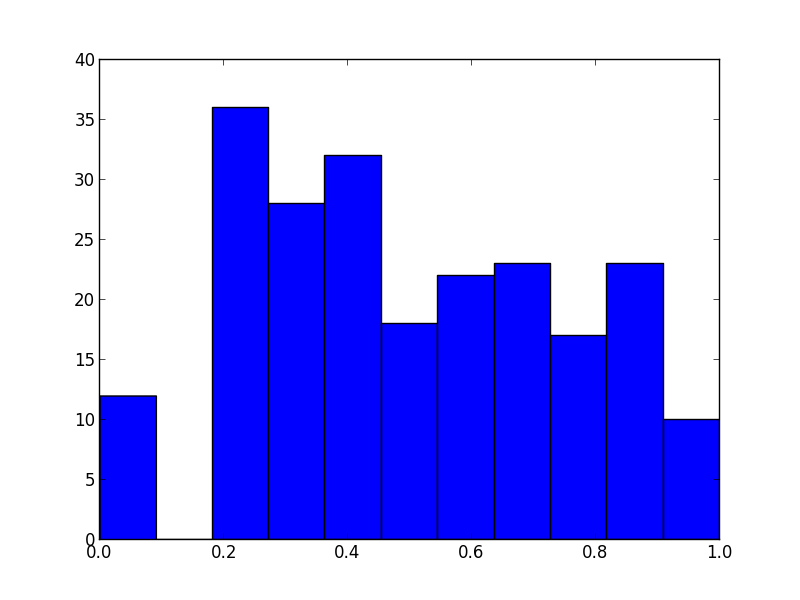
\includegraphics[width=0.5\textwidth]{images/github-popular.png}
\end{center}

\begin{center}
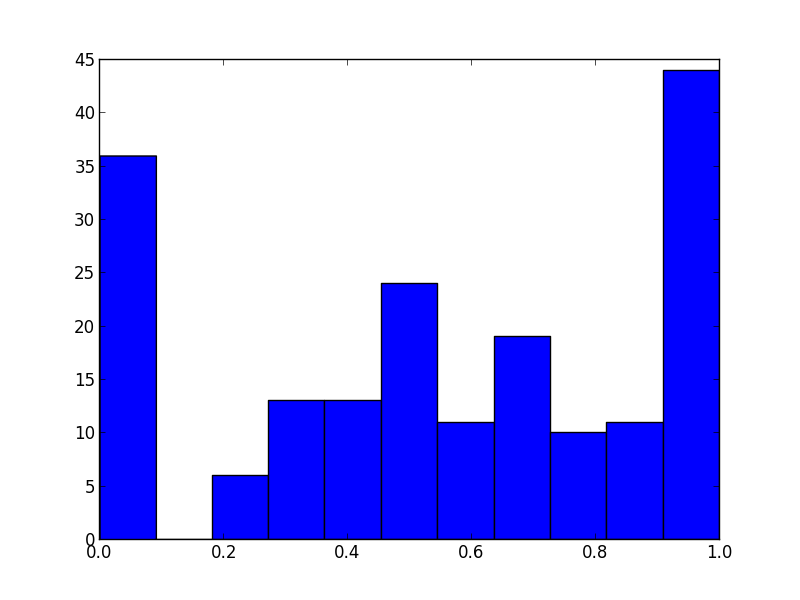
\includegraphics[width=0.5\textwidth]{images/github-unpopular.png}
\end{center}

\begin{center}
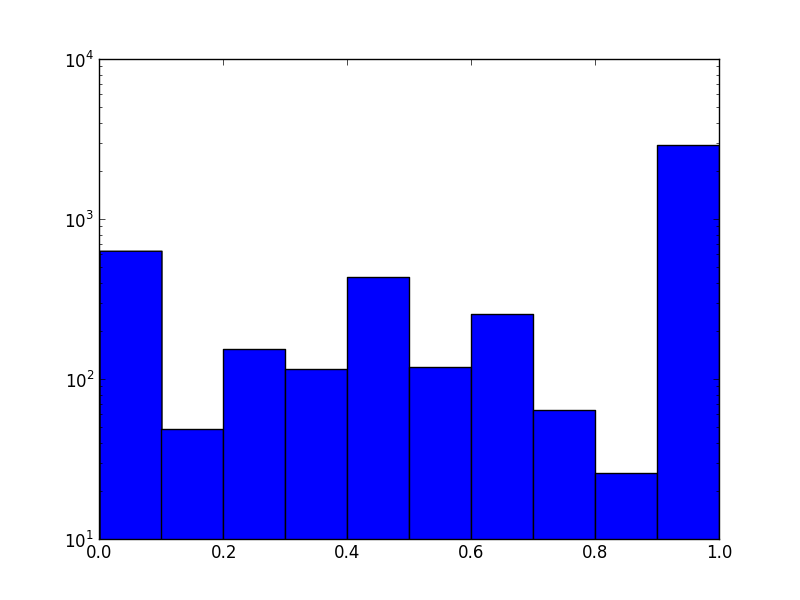
\includegraphics[width=0.5\textwidth]{images/github-q-histo.png}
\end{center}

\begin{center}
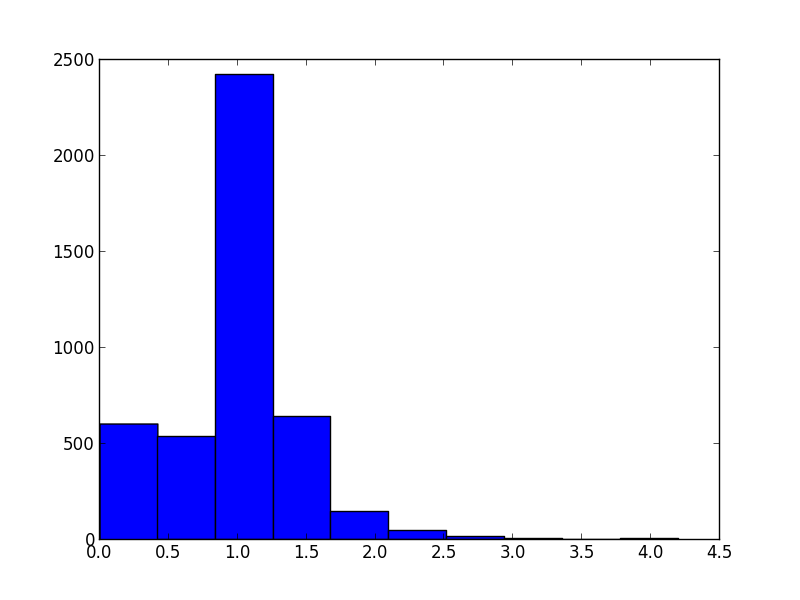
\includegraphics[width=0.5\textwidth]{images/github-smallworld-histo.png}
\end{center}

\begin{center}
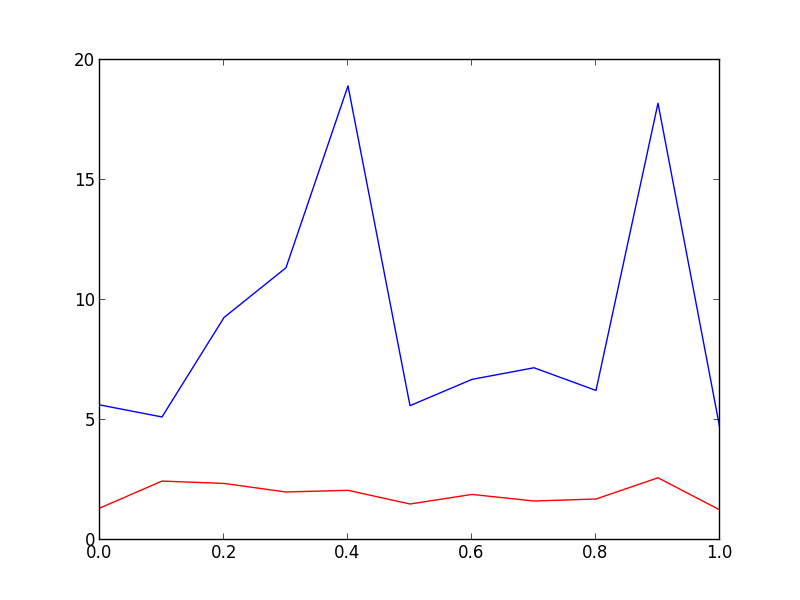
\includegraphics[width=0.5\textwidth]{images/github-graph.png}
\end{center}

\subsection{Qualitative}

\section{Conclusion}
\section{Acknowledgments}

\bibliographystyle{plain}
\bibliography{bibliography}


\end{document}